\pagestyle{ayllon}
\label{ayllon}

\hspace{.5cm}

\begin{center}
\hspace*{-2cm}\raisebox{5.5cm}{\rotatebox[origin=t]{90}{\Formular{\textbf{Lançamento}}}}
\hspace{1cm}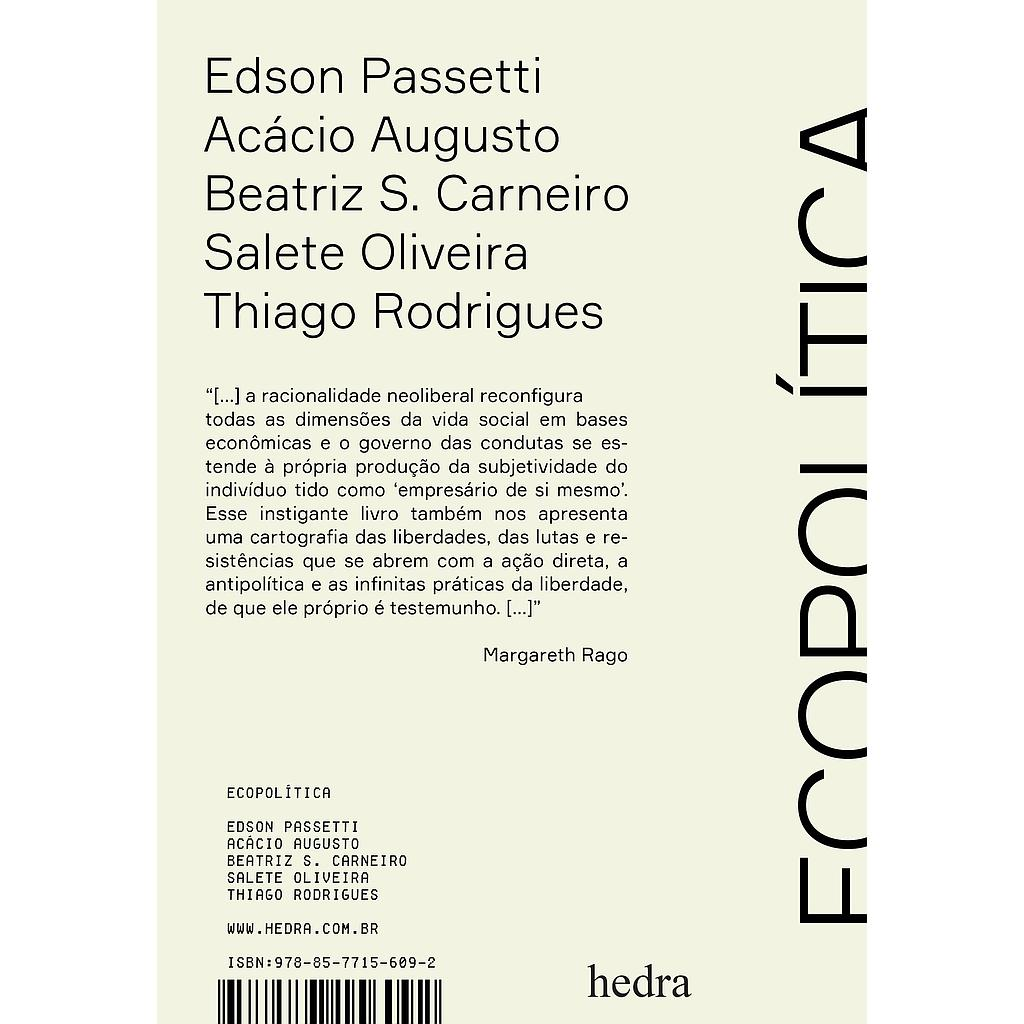
\includegraphics[width=60mm]{eco.jpeg}
\end{center}

\hspace*{-2cm}\_\_\_\_\_\_\_\_\_\_\_\_\_\_\_\_\_\_\_\_\_\_\_\_\_\_\_\_\_\_\_\_\_\_\_\_\_\_\_\_\_\_\_\_\_\_\_\_\_\_\_\_\_\_\_\_\_\_\_\_\_\_\_\_\_\_\_\_\_\_\_\_\_\_

\medskip

\noindent{}{\slsc{Cabalat shabat: poemas rituais}} reúne cinco textos, tratados aqui como poemas --- rezas e bênçãos judaicas --- e entoados na cerimônia de cabalat shabat, o recebimento do shabat a partir do pôr"-do"-sol da sexta"-feira. De teor místico, as canções são aqui apresentadas de maneira secular mas não anti"-religiosa. Em tradução do hebraico, sua temática situa"-se em paralelo a outros lugares poéticos da Antiguidade, trazendo no próprio ritual um entendimento estrutural e histórico do judaísmo. %442

\hspace{.5cm}

\hspace*{-.4cm}\begin{minipage}[c]{0.45\linewidth}
\small{
{\Formular{\textbf{
\hspace*{-.1cm}Título: Cabalat Shabat\\
Org.: Fabiana Grinberg\\ 
Editora: Ayllon\\
Páginas: 28\\
Formato: 17,1x26,7cm\\
Preço: R\$ 36,90\\
}}}}
\end{minipage}
\begin{minipage}[c]{0.50\linewidth}
\small{``Foram criados os céus e a terra e todos que lá vivem,/ a obra de Deus foi no sétimo dia concluída,/ e no sétimo dia contemplou-se toda a criação,/ e Deus abençoou o sétimo dia e o santificou.''}%,/ porque nele houve descanso de tudo o que havia sido criado.''} %244 
\end{minipage}

\pagebreak

\hspace{.5cm}

\begin{center}
\hspace*{-.5cm}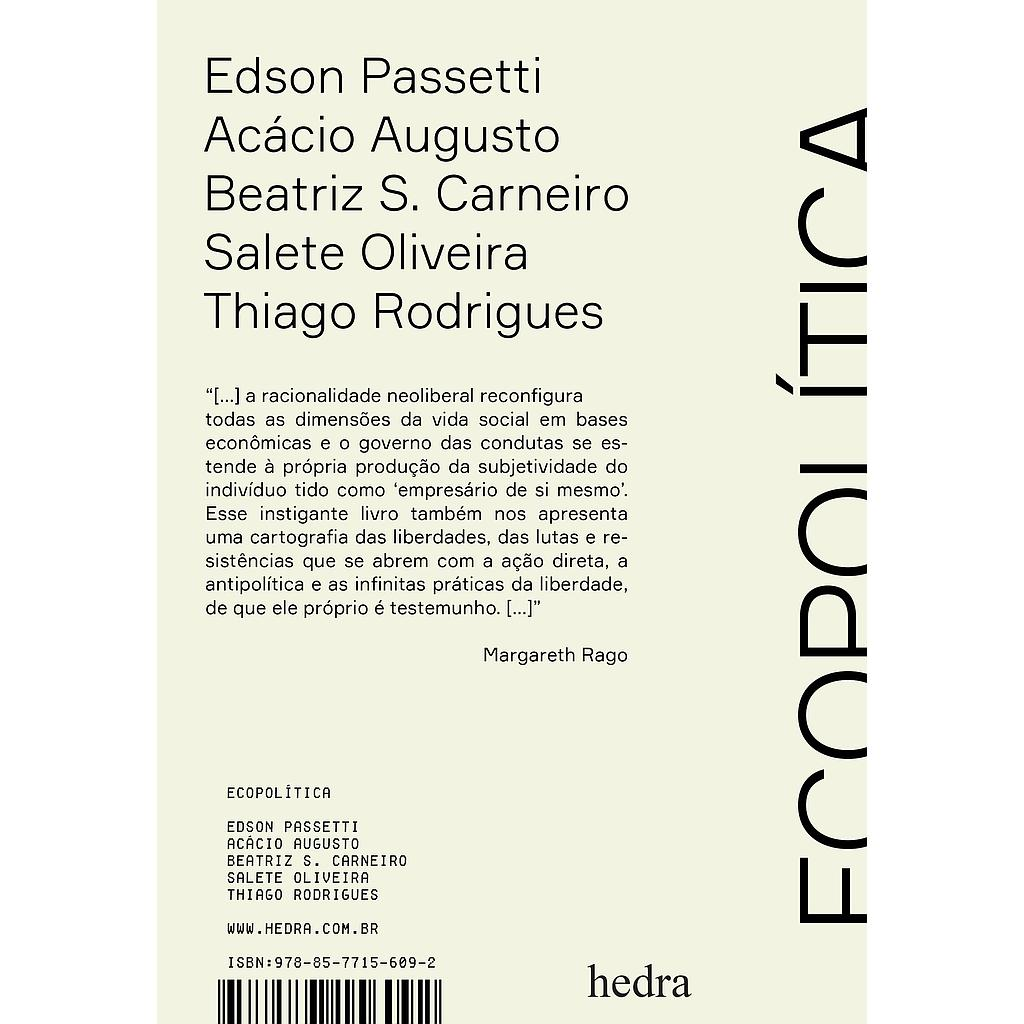
\includegraphics[width=60mm]{eco.jpeg}
%\hspace*{6cm}\raisebox{2cm}{\rotatebox[origin=t]{90}{\Formular{\textbf{Lançamento}}}}
\end{center}

\hspace*{-2cm}\_\_\_\_\_\_\_\_\_\_\_\_\_\_\_\_\_\_\_\_\_\_\_\_\_\_\_\_\_\_\_\_\_\_\_\_\_\_\_\_\_\_\_\_\_\_\_\_\_\_\_\_\_\_\_\_\_\_\_\_\_\_\_\_\_\_\_\_\_\_\_\_\_\_

\medskip

\noindent{}A narrativa de {\slsc{Fragmentos de um diário encontrado}} constituí"-se em torno da figura de alguém que se entrega aos labirintos urbanos parisienses em busca de algo tão perdido quanto indefinível: através das passagens desse diário o autor anônimo encarna o olhar do errante sobre a cidade. De 1932, a obra está afinada com o caráter rebelde das vanguardas artísticas europeias das décadas de 20 e 30 e com outros literatos romenos de seu tempo, como Cioran, Ionesco e Eliade.

\hspace{.5cm}

\hspace*{-.4cm}\begin{minipage}[c]{0.45\linewidth}
\small{
{\Formular{\textbf{
\hspace*{-.1cm}Título: Fragmentos de um diário encontrado\\
Autor: Mihail Sebastián\\ 
Editora: Ayllon\\
Páginas: 55\\
Formato: 11x18cm\\
Preço: R\$ 34,90\\
}}}}
\end{minipage}
\begin{minipage}[c]{0.50\linewidth}
\small{``Numa noite de novembro (em circunstâncias que não cabem aqui revelar) achei, na ponte Mirabeau, em Paris, um caderno de capa preta, lustrosa, de lona, igual àqueles que costumam ser usados nas mercearias como livro-caixa.''} 
\end{minipage}

\pagebreak
